%%%%%%%%%%%%%%%%%%%%%%%%%%%%%%%%%%%%%%%%%%%%%%%%%%%%%%%%%%%%%%%%%%
%%%%%%%% ICML 2013 EXAMPLE LATEX SUBMISSION FILE %%%%%%%%%%%%%%%%%
%%%%%%%%%%%%%%%%%%%%%%%%%%%%%%%%%%%%%%%%%%%%%%%%%%%%%%%%%%%%%%%%%%

% Use the following line _only_ if you're still using LaTeX 2.09.
%\documentstyle[icml2013,epsf,natbib]{article}
% If you rely on Latex2e packages, like most moden people use this:
\documentclass{article}

% For figures
\usepackage{graphicx} % more modern
%\usepackage{epsfig} % less modern
\usepackage{subfigure}
\usepackage{filecontents}
\newlength\myindent
\setlength\myindent{2em}
\newcommand\bindent{%
  \begingroup
  \setlength{\itemindent}{\myindent}
  \addtolength{\algorithmicindent}{\myindent}
}
\newcommand\eindent{\endgroup} 


% For citations
\usepackage{natbib}

% For algorithms
\usepackage{algorithm}
\usepackage{algorithmic}
%\usepackage{algpseudocode}
% As of 2011, we use the hyperref package to produce hyperlinks in the
% resulting PDF.  If this breaks your system, please commend out the
% following usepackage line and replace \usepackage{icml2013} with
% \usepackage[nohyperref]{icml2013} above.
\usepackage{hyperref}

% Packages hyperref and algorithmic misbehave sometimes.  We can fix
% this with the following command.
\newcommand{\theHalgorithm}{\arabic{algorithm}}

% Employ the following version of the ``usepackage'' statement for
% submitting the draft version of the paper for review.  This will set
% the note in the first column to ``Under review.  Do not distribute.''
%\usepackage{icml2013} 
% Employ this version of the ``usepackage'' statement after the paper has
% been accepted, when creating the final version.  This will set the
% note in the first column to ``Proceedings of the...''
\usepackage[accepted]{icml2013}


% The \icmltitle you define below is probably too long as a header.
% Therefore, a short form for the running title is supplied here:
\icmltitlerunning{Intelligent Texas Holdem No Limit PokerBot}

\begin{document} 

\twocolumn[
\icmltitle{Intelligent Texas Holdem No Limit PokerBot}

% It is OKAY to include author information, even for blind
% submissions: the style file will automatically remove it for you
% unless you've provided the [accepted] option to the icml2013
% package.
\icmlauthor{Srivatsan Srinivasan}{srivatsansrinivasan@g.harvard.edu}
\icmlauthor{Sebastien Baur}{sebastienbaur@g.harvard.edu}
\icmlauthor{Donghun Lee}{donghunlee@g.harvard.edu}

% You may provide any keywords that you 
% find helpful for describing your paper; these are used to populate 
% the "keywords" metadata in the PDF but will not be shown in the document
\vskip 0.3in
]

\begin{abstract} 
To deal with the challenges posed by imperfect information games, we propose a poker-bot that understands implicit features through a combination of self-play with deep reinforcement learning. For the learning agent, we propose to use the architecture of NFSP (Neural Fictitious Self Play) where each playing agent stores separate experience buffers and trains two neural networks, one which learns best action values using off-policy reinforcement learning and another, which maps states to action probabilities and hence learns, the agent's average strategy. We also employ sub-networks that learn abstracted states using player hand strength and (potentially) a Bayes Net that infers the distribution of opponent hands from the betting actions, whose outputs feed into the master network. We plan to sequentially test the agent's performance against a random agent, a fixed policy agent and finally, commercial AI agents.
\end{abstract} 
\section{Introduction}
\label{intro}
Poker is a quintessential game of imperfect information. The challenges involved in poker include sophisticated decision sequences, large state-action space, imperfect information and adversarial behavior, presenting a perfect template for  probabilistic inference and reinforcement reinforcement learning that employ neural networks to interpret complicated non-linearities.

Heads-up no-limit Texas Holdem (HUNL) is a two-player version of poker in which two cards are initially dealt face down to each player(pre-flop), and additional cards are dealt face up in three subsequent rounds(flop,turn and river). No limit is placed on the size of the bets although there is an overall limit to the total amount wagered in each game. Imperfect information games require more complex reasoning than similarly sized perfect information games. The correct decision at a particular
moment depends upon the probability distribution over private information that the opponent holds, which is revealed through their past actions. However, how our opponents actions reveal that information depends upon their knowledge of our private information and how our actions reveal it. This kind of
recursive reasoning is why one cannot easily reason about game situations in isolation, which is at the heart of heuristic search methods for perfect information games.

\section{Background}
\subsection{Reinforcement Learning}
Reinforcement learning (Sutton and Barto, 1998) agents typically learn to maximize their expected
future rewards from interaction with an environment. The environment is usually modeled as a
Markov decision process (MDP), where the agent tries to learn an optimal stochastic action policy in each state that maximizes its total expected gain in a trajectory. Many reinforcement learning algorithms learn from sequential experience in the form of transition tuples $(s_t; a_t; r_{t+1}; s_{t+1})$. A common objective is to learn the action-value function, Q(s,a)- value of taking an action from a state and staying on course with the base policy further, in an off-policy setting where you learn from the experiences of other policies too. Q-Learning(Watkins and Dayan,1992) is an algorithm mostly to this effect where we learn from a batch of transitions. DQN with experience replay(Mnih et al., 2015) are recent advancements in Q-learning where the agent learns Q-values from experience data by fitting neural networks in the state-action space.
\subsection{Nash Equilibrium and Fictitious Self-Play}
Extensive-form games are a model of sequential interaction involving multiple players. Assuming
rationality, each player’s goal is to maximize his payoff in the game. Each player chooses a behavioural
strategy that maps information states to probability distributions over available actions. A strategy profile $\pi$ = $(\pi_1;... ; \pi_n)$ defines a collection of strategies for all players. A Nash equilibrium is a strategy profile such that each player’s strategy in this profile is a best response to the other strategies. Similarly, an approximate or $\epsilon$-Nash equilibrium is a profile of $\epsilon$ - best responses, responses which are not sub-optimal by more than $\epsilon$. Fictitious play (Brown, 1951) is a game-theoretic model of learning from self-play. Fictitious players choose best responses to their opponents’ average behaviour. The average strategies of fictitious players approximately converge to Nash equilibria(Leslie and Collins, 2006) and allows for approximate best responses and perturbed average strategy updates, making it particularly suitable for machine learning. (Bowling and Veloso, 2001) prove that Nash equilibria are the only strategy profiles that rational agents can hope to converge on in self-play. 
\section{State-Action Space Representation}
\subsection{State Space}
The cards are one-hot-encoded arrays. The board and the player's hand are separated so that they private and public information can be processed differently The board is decomposed in 3 parts (for 3 betting rounds), so that the neural network can process each part with the actions that were taken in
a given betting round. We also take into account the actions that were taken in a given episode. They are represented as a 4x5x6x2 array (4 betting rounds, 5 types of action, at most 6 bets per player in a given betting round, 2 players).  The action representation encodes allowed actions such as bet, call, check, going all-in, raise. To bound the possible number of actions per betting round, we forbid the players to do more two min-raise by betting round (after 2 they have to double). A last array contains the blinds, money stacks, pot, and dealer button values.
\subsection{Hand Strength Evaluation}
The number of possible combinations in the aforementioned state space representation is humongous and hence, the learning problem becomes computationally intractable. We resort to the structure of the game in order to implicitly cluster the state-action possibilities based on possible outcomes. For instance, consider an extreme case of a board that has {Ah, Ad, Qh, Jd, Kd} and assume the agent has two non-face cards that don't form a pair. Irrespective of the the cards' numerical value, the agent is expected to take the same action in the game, which implicitly reduces potentially a ${10}\choose{2}$ hole cards possibilities into a single point estimate. We intend to capture this intuition through  hand strength evaluation. With h being the set of hole cards and b being the set of board cards, HS(h,b)is defined as follows. Here, p(w) is the probability of the agent winning the game(assuming a final showdown) and the games being simulated through 100000 Monte Carlo simulations(w ith opponent cards and remaining portion of board being randomly sampled) for each combo of cards. $p(s_i)$ similarly suggests the probability of obtaining different final hands( Straight, flush etc.) from the current hole and board under MC simulations.
\[HS(h,b) = \Bigl[ p(w^{(hb)}), p(s_1^{(hb)}), ... p(s_n^{(hb)}) \Bigr ]\]
\subsection{State Abstraction through NN}
We calculate the hand strengths of the pre-flop, flop, turn and river(trivial) cards using the methodology suggested above. Since the number of combinations is pretty huge(O($10^7$)), we created a lookup table for the hand strength of these combinations. Then we build a fully-connected neural network that utilizes the hand strength evaluation table as the labeled dataset in order to predict these metrics, given a set of hole and board cards. The output of this NN is fed into our master NFSP network(to follow). Our Q network has an auxiliary output that tries to predict the hand strength based only on the board and the cards, so that similar situations get represented similarly at the last hidden layer of this sub-network - a representation that is then used to predict the Q values.
\section{Neural Fictitious Self-Play(NFSP)}
\subsection{Prioritized Experience Replay}
In the Reinforcement Learning setting, RL agents incrementally update their parameters (of the policy,
value function or model) while they observe a stream of experience. In their simplest form, they
discard incoming data immediately, after a single update. Two issues with this are (a) strongly
correlated updates that break the i.i.d. assumption of many popular stochastic gradient-based algorithms,
and (b) the rapid forgetting of possibly rare experiences that would be useful later on. Experience replay (Lin, 1992) addresses both of these issues: with experience stored in a replay memory, it becomes possible to break the temporal correlations by mixing more and less recent experience for the updates, and rare experience will be used for more than just a single update. This was demonstrated in the Deep Q-Network (DQN) algorithm (Mnih et al., 2013; 2015), which stabilized the training of a value function, represented by a deep neural network, by using experience replay.

Here we use a modified version of experience replay, called PER - Prioritized Experience Replay((Schaul et.al., 2016)for storing our transition buffers. PER samples from the experience buffer with higher probability weight to transitions with larger TD error. The two classic approaches would include a proportional probability weighting scheme and a rank-based probability weighting scheme. Since the proportional weighting scheme is sensitive to outliers at times, we go ahead with the rank-based weighting scheme, where each transition is as probable as the inverse rank of TD-error. We use the same architecture for our RL buffer and SL buffer in the NFSP algorithm which follows.

\subsection{NFSP}
NFSP(Heinrich and Silver, 2016) combines FSP with neural network function approximation. In algorithm 1 all players of the game are controlled by separate NFSP agents that learn from simultaneous play against each
other, i.e. self-play. An NFSP agent interacts with its fellow agents and memorizes its experience
of game transitions and its own best response behaviour in two memories,$M_{RL}$ and $M_{SL}$. NFSP
treats these memories as two distinct datasets suitable for deep reinforcement learning and supervised
classification respectively. The agent trains a neural network, $Q(s;a | \theta^Q)$, to predict action values from data in $M_{RL}$ using off-policy reinforcement learning. The resulting network defines the agent’s approximate best response strategy, $\epsilon$-greedy(Q), which selects a random action with probability $\epsilon$ and otherwise chooses the action that maximizes the predicted action values. The agent trains a separate neural network, $\Pi(s;a |\theta^{\Pi})$, to imitate its own past best response behaviour using supervised classification on the data in $M_{SL}$. This network maps states to action probabilities and defines the agent’s average strategy, $\pi = \Pi$. During play, the agent chooses its actions from a mixture of its two strategies $\beta$ and $\Pi$.

If we want all agents to learn simultaneously while playing against each other, we face the following
dilemma.In principle, each agent could play its average policy, $\Pi$, and learn a best response with off-policy Q-learning, i.e. evaluate and maximize its action values, $Q_i(s; a)$ of playing its best response policy $\beta_i$ against its fellow agents’ average strategy profile, $\Pi_{-i}$. However, in this case the agent would not generate any experience of its own best response behaviour, which is needed to train its average policy network that approximates the agent’s average of past best responses. Hence, NFSP agents choose their actions from the mixture of these policies. This enables each agent to compute an approximate best response, $\beta_i$, to its opponents’ anticipated average strategy profile by iteratively evaluating and maximizing its action values. Additionally, as each agent’s own best response policy is now sampled in proportion to the anticipatory parameter, they can now train their average policy networks from that experience.
\begin{algorithm}
   \caption{Neural Fictitious Self-Play}
   \label{alg:example}
   \begin{algorithmic}
   \STATE Initialize game G with 2 players. 
   \STATE Execute each player via runAgent.
   \STATE {\bfseries function} runAgent(G): 
   \bindent
   \STATE Initialize replay memories $M_{RL}, M_{SL}$ 
   \STATE Initialize action-value network $Q(s,a|\theta^Q)$
   \STATE Initialize average-policy network $\Pi(s,a|\theta^{\pi})$
   \STATE Initialize anticipatory hyper-parameter $\eta$  
   \STATE Define ${L_{SL}}$ as Softmax loss on $\pi$
   \STATE Define ${L_{RL}}$ as TD Error loss on Q value.
   \FOR{each episode}
   \STATE $\sigma $: P($\sigma$ = $\epsilon$ greedy Q ) = $\eta$, else $\sigma$ = $\Pi$ 
   \STATE Observe $s_1, r_1$
   \FOR{t=1,T}
   \STATE Sample action at from policy $\sigma$
   \STATE Execute $a_t$ and Observe $r_{t+1},s_{t+1}$
   \STATE Store $(s_t,a_t,r_{t+1},s_{t+1}$ in $M_{RL})$
   \IF{$ \sigma = \epsilon$ greedy Q} 
   \STATE Store $(s_t,a_t)$ in $M_{SL}$
   \ENDIF
   \STATE Update $\theta^{\Pi}$ with SGD on loss $L_{SL}$
   \STATE Update $\theta^{Q}$ with SGD on loss $L_{RL}$ 
   \ENDFOR
   \ENDFOR
   \eindent
  
   \end{algorithmic}
\end{algorithm}
\section{Bayesian Opponent Modeling}

If further time permits, we are also thinking of Bayesian modeling of opponent hands - an inference problem which suggests the distribution over opponent hands based on the game's action transitions. The output of this inference could be used to train the master neural network as we expect to see more robust results with an approximate idea on the most likely types of opponent hands. As a follow-up, we bucket the expected hand strength distributions into k buckets. Intuitively, it makes more sense to cluster these distributions into buckets in an exponentially decreasing fashion, meaning really strong hands should be composed of very few set of cards.\\
\begin{figure}
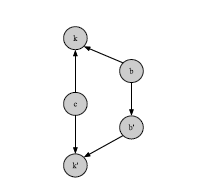
\includegraphics[scale=1]{Bayes_opp.png}
\caption{Graphical Model of the hand transitions}
\label{fig:fig1}
\end{figure}

We can intuitively think of the hidden hand strength as dependent on cards, board and opponent actions. From this, as first step, we can marginalize over all possible actions(call,fold,raise) to get a graphical model that depends on board and cards as shown in Figure \ref{fig:fig1}.The graphical model in shows us that in each state, hand strength k is a mixture of both the opponents' cards c and the board cards b.  With this dataset, we can perform inference on the expected hand strength bucket of the opponent, which would be used as an input to train the Q-network. Again,as outlined earlier, this will be an optional effort based on the availability of time.
\section{Status Report}
We have completed the following pieces as on 11/18.
\subsection{Current Progress}
\begin{enumerate}
\item Hand Strength Evaluator has been completed and look-up tables for pre-flop, flop and river have been generated and saved.
\item An end-to-end simulator/game play engine has been built and tested with intuitive cases and with random agents, fixed policy agents.
\item The Q-network has been setup using the following features - hole cards, board cards, action history, pot and dealer information.
\item The average policy network for the NFSP has been setup using the same base features and it shares multiple layers with the previous NN while diverging in a few others.
\item Prioritized experience replay buffers have been built for both the Q network and the average policy network and have been integrated with the main networks.
\end{enumerate}
\subsection{Next Milestones/Deliverables}
As next steps, we propose to focus on the following items in the same order of priority.
\begin{enumerate}
\item Training the neural network - We have to train the integrated neural network on the NFSP simulations and assert if the agent learns meaningful weights within sane times.
\item The convergence and testing results of the Q-network need to be derived from training and documented. 
\item Basic Evaluation - Once trained, we need to evaluate the performance of the RL agent against dumb agents such as random action agent and fixed policy agent in order to assert basic sanity.
\item Evaluation against commercial AI - We need to let the agent play against commercial pokerbots and understand its performance dynamics.
\item Having laid out the basic structure of the opponent model, we need to build the model and test it once the agent begins training. 
\end{enumerate}
\end{document} 


